\chapter{Demoversion toiminta ja analyysi}
\label{ch:projektin-lähtökohdat}
Diplomityön tekijä ennen tämän työn aloitusta oli kehittänyt ohjelmiston, joka kykeni viestien tilaukseen ja tallentamiseen. Ohjelma oli tarkoitettu demoksi tai prototyyppiksi ennen varsinaista toteutusta. Demon tarkoituksena oli opettaa tekijää IEC 61850 -standardin suhteen, todentaa viestien tilaamisen mahdollisuus ja tuoda esille toteutukseen liittyviä ongelmia. Ohjelma kykeni tilaamaan viestejä yhden IED-laitteen kaikilta RCB-instansseilta, prosessoimaan viestit ja tallentamaan ne relaatiotietokantaan.

Demoa ei ollut mahdollista käyttää tuotannossa osana muuta järjestelmää, sen arkkitehtuurin ja toiminnan epävarmuuden takia. Tässä kappaleessa käydään läpi demon toimintaa ja siihen liittyviä ongelmia. Demosta on tarkoitus analysoida sen toiminnan epävarmuutta ja saada selville mistä ne mahdollisesti johtuivat. Näitä tietoja käytetään myöhemmin apuna uuden version suunnittelussa.


\section{Arkkitehtuuri}
\label{ch:demoversio-ja-sen-toiminta}
Demoversio oli ohjelmoitu Ruby-ohjelmointikielellä. Kuvassa \ref{fig:demo-architecture} on esitetty demoversion arkkitehtuuri korkealla tasolla ja kuinka viesti IED-laitteelta siirtyy tietokantaa. Yksi ajettu demoversion prosessi pystyi tilaamaan yhden IED-laitteen kaikki RCB-luok\-ki\-en instanssit. Instanssien tiedot luettiin relaatiotietokannasta. Ohjelmisto prosessoi viestit ja tallensi ne relaatiotietokantaan myöhempää käyttöä varten. Ruby-ohjelmistossa tärkeässä osassa oli \emph{libIEC61850}-kirjasto \cite{libIEC61850-homepage}. libIEC61850-kirjasto on avoimen lähdekoodin C-kielellä toteutettu kirjasto, joka abstrahoi IEC 61850 -standardin matalan tason määrittämiä palvelukutsuja ja datarakenteita helppokäyttöiseksi rajapinnaksi. Kirjasto tarjosi toiminnallisuuden IED-laitteella olevan palvelinohjelmiston, sekä IED-laitetta käyttävän asiakasohjelmiston toteuttamiseen. IED-laitteen palvelimelle kirjasto tarjosi funktioita ja rakenteita standardin määrittämien luokkien hierarkian rakentamiseen ja käsittelyyn. IED-laitteen asiakasohjelmalle kirjasto tarjosi funktioita ja rakenteita standardin määrittämiin palveluihin, kuten arvojen lukuun ja asettamiseen, datajoukkojen käyttöön ja viestien tilaamiseen. Demoa toteutettiin oikeaa IED-laitetta vasten, joten kirjastosta käytetiin vain sen asiakasohjelman ominaisuuksia. Demon toteutuksen aikana kirjasto todettiin hyväksi vaihtoehdoksi ja sitä päätettiin käyttää myös uuden version toteutuksessa.

\begin{figure}[ht!]
	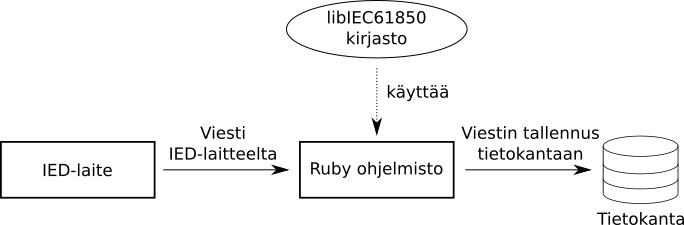
\includegraphics[width=1\textwidth]{pictures/demo-architecture.png}
	\caption{Ruby:lla toteutetun demoversion arkkitehtuuri ja tiedonsiirto.}
	\label{fig:demo-architecture}
\end{figure}

LibIEC61850-kirjasto on rakennettu käyttämään MMS-protokollaa tiedonsiirrossa IED-laitteen ja sen asiakasohjelman välillä IEC 61850 -standardin 8-1 osan mukaan. Kuvassa \ref{fig:libiec61850-layer-architecture} on esitetty kirjaston kerrosarkkitehtuuri asiakasohjelmalle. Kirjastoon on toteutettu \emph{laiteabstraktiokerros} (engl. \emph{Hardware Abstraction Layer}, lyhennetään \emph{HAL}). HAL:in avulla kirjasto voi toimia monella eri laitealustalla, ja käyttäjä voi tarvittaessa lisätä oman HAL-implementaation. Demoversiota suoritettiin Linux-käyttöjärjestelmällä, joten kirjastosta käytettiin olemassa olevaa Linux HAL -toteutusta. Kuvassa \ref{fig:libiec61850-layer-architecture} on punaisella merkitty laatikot, jotka kirjaston käyttäjä voi tarjota itse, keltaisella kirjaston uudelleenkäytettävät MMS-protokollan osuudet ja sinisellä IEC 61850 -standardin toteuttavat osuudet. Kuvaan on merkitty vihreällä demoon toteutetut osuudet, eli Ruby-kielelle liitos C-kieleen ja tämän päälle Ruby:lla toteutettu ohjelmisto.

\begin{figure}[ht!]
	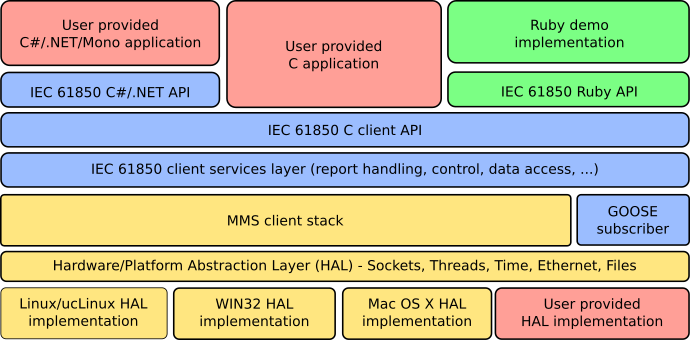
\includegraphics[width=1\textwidth]{pictures/libiec61850-layer-architecture.png}
	\caption{libIEC61850-kirjaston kerrosarkkitehtuurin komponentit, vihreällä Ruby toteutukseen lisätyt osat (pohjautuu kuvaan \mbox{\cite{libIEC61850-api-overview}}).}
	\label{fig:libiec61850-layer-architecture}
\end{figure}

Ruby-koodista C-kielen funktioiden kutsuminen ei ole suoraan mahdollista, vaan kielten väliin täytyy toteuttaa liitos. Demoversiossa liitos oli tehty käyttäen Ruby:lle saatavaa \emph{ruby-ffi}-kirjastoa \cite{ruby-ffi-repo} (engl. \emph{Foreign Function Interface}, lyhennetään \emph{FFI}). Liitoksen avulla Ruby voi kutsua C-kielen funktioita ja käyttää sen struktuureita ja muuttujia. Demossa kirjasto huolehti matalan tason IEC 61850 asiat, ja Ruby-osuus keskittyi liitoksen avulla viestien tilaamiseen, käsittelyyn ja tallentamiseen.


\section{Toiminta}
\label{ch:ongelmakohdat-ja-analysointi}
Ohjelman toiminta on esitetty sekvenssikaavioissa \ref{fig:sequence-diagram-report-subscription} ja \ref{fig:sequence-diagram-report-subscription-processing}. Sekvenssikaavio \ref{fig:sequence-diagram-report-subscription} jatkuu kuvassa \ref{fig:sequence-diagram-report-subscription-processing}. Kuvissa ohjelman kaksi eri silmukkaa on esitetty loop-laatikoilla. Sekvenssikaaviossa osallisena ovat tietokanta, Ruby-ohjelma, libIEC61850-kirjasto, libIEC61850-kirjaston natiivisäie ja IED-laitteen palvelinohjelma. Kirjaston natiivisäie on vastuussa yhteyden ylläpidosta ja datan siirtämisestä IED-laitteen ja kirjastoa käyttävän prosessin välillä. Sekvenssikaavioon on merkitty paksulla suorituksessa olevat palkit, esimerkiksi IED-laitteen palvelinohjelmisto on koko ajan suorituksessa. Kuvissa kaikki kohdat on numeroitu ja näihin viitataan tulevassa tekstissä.

IED-laiteella viestejä mahdollisesti generoidaan ja lähetetään samaan aikaan. Seurauksena niitä voi saapua libIEC61850-kirjastolle ennen kuin edellinen viesti on käsitelty. Tätä varten kirjasto toteuttaa sisäisen puskurin viestien vastaanottamiseen. Puskurista prosessoidaan seuraava viesti kun edellinen on prosessoitu. Toisin sanoen kirjasto ottaa viestejä vastaan sitä mukaan kun ne saapuvat ja ottaa niitä puskurista yksi kerrallaan saapumisjärjestyksessä. Kirjasto varaa yhden puskurin avattua yhteyttä kohti. Jos ohjelma avaa vain yhden yhteyden, kirjaston käyttäjän ei tarvitse huolehtia rinnakkaisuudesta. \cite{libIEC61850-repo}

\begin{figure}
	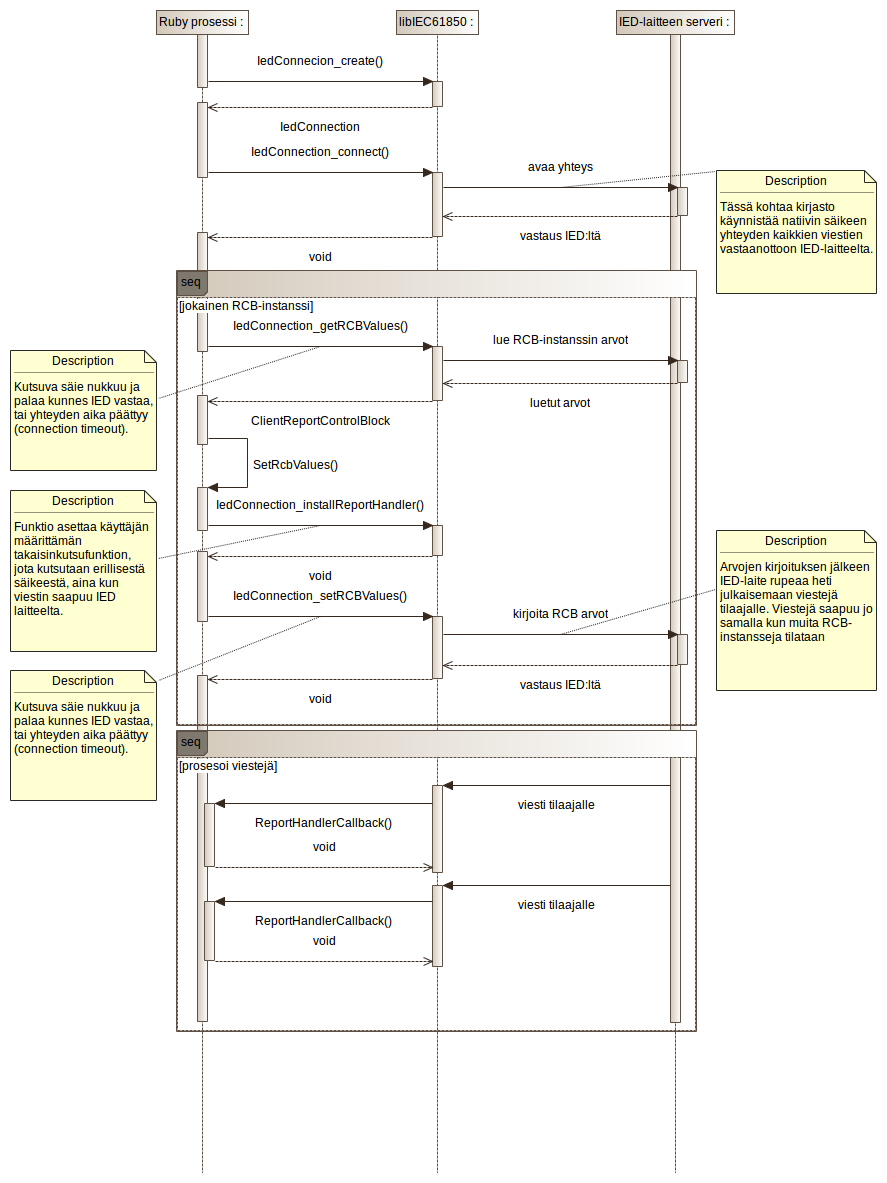
\includegraphics[width=1\textwidth]{pictures/sequence-diagram-report-subscription.png}
	\caption{Sekvenssikaavio kuinka Ruby-ohjelma avaa yhteydet ja tilaa kaikki IED-laitteen RCB-instanssit (jatkuu kuvassa \ref{fig:sequence-diagram-report-subscription-processing}).}
	\label{fig:sequence-diagram-report-subscription}
\end{figure}

\begin{figure}
	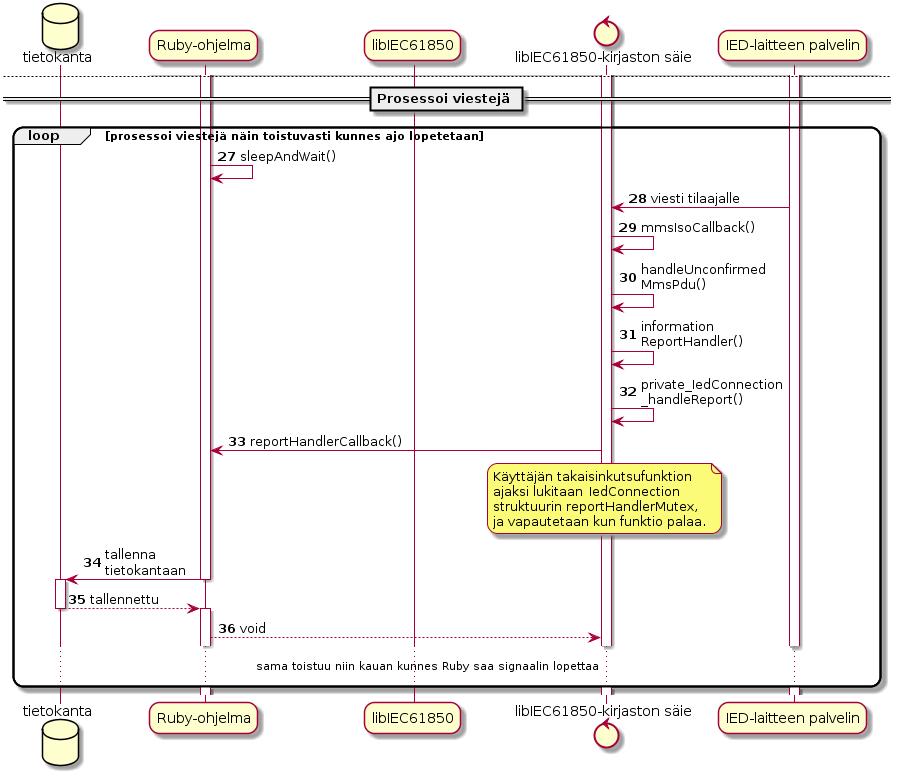
\includegraphics[width=1\textwidth]{pictures/sequence-diagram-report-subscription_001.png}
	\caption{Sekvenssikaavio kuinka Ruby-ohjelma prosessoi ja tallentaa viestejä libIEC61850-kirjastoa käyttäen (jatkoa kuvalle \ref{fig:sequence-diagram-report-subscription}).}
	\label{fig:sequence-diagram-report-subscription-processing}
\end{figure}

Ensimmäisenä ohjelma luki tietokannasta IED-laitteen, sekä sen kaikki RCB-instanssien tiedot. Tämän avulla ohjelma tiesi mikä IED-laitteen IP-osoite on ja mitkä olivat RCB-instanssien viitteet (kohdat 1--2). Tämän jälkeen ohjelma pystyi muodostamaan yhteyden IED-laitteelle tekemällä instanssin \texttt{IedCon\-nec\-ti\-on} struktuurista funktiolla \texttt{Ied\-Con\-nec\-ti\-on\_crea\-te\-()} (kohdat 3--4). Tämän jälkeen struktuuri annetaan \texttt{Ied\-Con\-nec\-ti\-on\-\_\-con\-nect\-()} funktiolle, joka avaa yhteyden IED-laitteelle ja palaa vasta kun vastaus saapuu (kohdat 5--11). Tässä vaiheessa libIEC61850-kirjasto käynnistää erillisen natiivisäikeen yhteyden viestien vastaanottoon. Tätä säiettä kirjasto käyttää tulevien viestien vastaanottoon ja lähettämiseen. Yhteyden avauksen jälkeen jokainen RCB-instanssi tilataan lukemalla ensin sen arvot IED-laitteelta funktiolla \texttt{Ied\-Con\-nec\-ti\-on\-\_\-get\-RCB\-Va\-lu\-es\-()} (kohta 12). Funktiokutsu nukkuu ja palaa vasta kunnes erillinen säie ilmoittaa, että vastaus on saapunut tai yhteyden aika ylittyy. Kirjaston funktio  \texttt{send\-Re\-qu\-est\-And\-Wait\-For\-Res\-pon\-se\-()} nukkuu ja odottaa vastausta (kohdat 13--16). RCB-arvot luettuaan, kirjasto palauttaa struktuurin \texttt{Cli\-ent\-Re\-port\-Cont\-rol\-Block}, joka sisältää luetut tiedot RCB-instanssista (kohta 17). Samaa struktuuria käytetään arvojen muuttamiseen ja niiden takaisin kirjoittamiseen IED-laitteelle. Ennen muunneltujen RCB-arvojen takaisin kirjoittamista ja viestien tilaamista, täytyy kirjastolle asettaa takaisinkutsufunktio, jota kirjasto kutsuu aina kun tilattu viesti saapuu IED-laitteelta. Takaisinkutsufunktioksi asetetaan funktiolla \texttt{Ied\-Con\-nec\-ti\-on\-\_\-ins\-tall\-Re\-port\-Hand\-ler\-()} (kohdat 19--20). Asetuksen ajaksi kirjasto lukitsee \texttt{re\-port\-Hand\-ler\-Mu\-tex}:in. Tätä samaa lukitusta käytetään kun viesti takaisinkutsufunktiota kutsutaan viestin saapuessa (kohdat 33--36). Tilanteessa jossa takaisinkutsufunktiota asetetaan samalla kun viesti on saapunut, joutuu toinen osapuoli odottamaan lukituksen vapautumista. Tämän jälkeen arvot kirjoitetaan takaisin IED-laitteelle funktiolla \texttt{Ied\-Con\-nec\-ti\-on\-\_\-set\-RCB\-Va\-lu\-es\-()} (kohdat 21--26). Tämä funktio palaa vasta kun IED vastaa tai yhteyden aika ylittyy. Heti arvojen kirjoitusten jälkeen IED aloittaa lähettämään viestejä tilaajalle. Eli samalla kun muita RCB-instansseja tilataan, tilatut RCB-instanssit lähettävät jo viestejä ja aiheuttavat takaisinkutsufunktion suorittamisen. Kun kaikki RCB-instanssit on tilattu, ohjelma jää viimeiseen silmukkaan odottamaan ja prosessoimaan viestejä (kohdat 27--36). Kun viesti saapuu, säie kutsuu ensin sisäisesti \texttt{mms\-I\-so\-Call\-back\-()} funktiota, joka kutsuu muita kirjaston sisäisiä funktioita ja lopuksi asetettua takaisinkutsufunktiota (kohdat 28--33). Takaisinkutsufunktio on liitetty Ruby-funktioon, joka tallentaa raportin tiedot tietokantaan (kohdat 33--36). Ruby-funktion suorituksen ajaksi kirjasto lukitsee \texttt{re\-port\-Hand\-ler\-Mu\-tex}:in, ja vapautetaan kunnes Ruby-funktion suoritus palaa. Tätä jatkuu niin kauan kunnes ohjelmalle lähetetään jokin signaali joka lopettaa sen suorituksen. \mbox{\cite{libIEC61850-repo}}


\section{Ongelmien analyysi}
Demo oli toteutettu käyttäen \emph{Ruby on Rails} -kehystä, lyhennetään \emph{RoR}. RoR on tarkoitettu web-sovellusten kehittämiseen Ruby-kielellä. Demo toteutettiin suoritettavaksi RoR:in tarjoamalla Ruby-koodin suorituksen mekanismillä \cite{rails-runner}. Mekanismi sallii Ruby-koodin suorituksen RoR:in kontekstissa. Konteksti salli järjestelmän kirjastojen ja koodien käytön demossa. Huonona puolena tässä oli, että yksinkertaisen ohjelman suoritus vaatii järjestelmän kontekstin muistiin lataamisen ennen suoritusta. Tästä seurauksena yksi suoritettu demon prosessi varasi muistia noin 150 Mt, verrattuna uuteen RoR-projektiin, joka vei noin 67 Mt muistia. Ohjelman yksinkertaisuuteen nähden varatun muisti määrä on suuri ja sitä olisi mahdollista pienentää.

Demossa isoimpana ongelmana oli sen huono suorituskyky ja toiminnan epävarmuus RCB-instanssien määrän ollessa enemmän kuin muutama. RCB-instanssien määrän ollessa liian suuri ohjelma saattoi epäonnistua osan tilaamisessa, koska yhteys aikakatkaistiin arvojen kirjoituksessa tai luvussa. Lisäksi ongelmaksi muodostui usean RCB instanssin tilaamisen kulunut aika. Yhteensä aikaa saattoi kulua noin 30 sekuntia 10 instanssien tilaamiseen.

Huonoon suorituskykyyn oli syynä muutama asia. Yksi niistä oli Ruby-kielen huonompi suorituskyky verrattuna natiivisti käännettyyn C-kieleen. Ruby on tulkattava kieli kuten esimerkiksi Python, joka tulkataan rivi kerrallaan ja suoritetaan. Lähdekoodia ei käännetä kokonaan ensin konekäskyiksi erillisellä kääntäjällä, kuten C-kielessä. Valmiiksi käännetty lähdekoodi tarvitsee vain ajaa, kun taas tulkattavassa kielessä rivi täytyy ensin tulkata ja sitten ajaa. Ruby:ssa käytettiin sen oletustulkkia \emph{MRI/YARV} (engl. \emph{Matz's Ruby Interpreter}, lyhennetään \emph{MRI} tai \emph{Yet another Ruby VM}, lyhennetään \emph{YARV}). Ruby versiosta 1.9 eteenpäin käyttää YARV-tulkkia. Toinen syy oli Ruby-kielen oletustulkissa oleva \emph{globaali tulkkilukitus} (engl. \emph{Global Interpreter Lock}, lyhennetään \emph{GIL}, tai \emph{Global Virtual Machine Lock}, lyhennetään \emph{GVL}). GIL pakottaa Ruby-ohjelman ajoon vain yhdellä ytimellä ja vain yksi säie vuorossa kerrallaan ja on täysin riippumaton käyttöjärjestelmän vuorottajasta \mbox{\cite[s.~131--133]{Odaira2014}}. Kuvassa \ref{fig:ruby-gil} on esitetty kuinka Ruby-tulkki vuorottaa kahta ajossa olevaa säiettä. Kuvassa demon Ruby-koodi kutsuu \texttt{Ied\-Con\-nec\-ti\-on\-\_\-set\-RCB\-Va\-lu\-es\-()} funktiota, ajo jää kesken ja tapahtuu vaihto, koska viesti saapui. Takaisinkutsufunktio suoritetaan ja suoritus palaa takaisin aikaisempaan funktion suoritukseen. Tässä vaiheessa jos vaihto on huonolla hetkellä ja kesti liian kauan, tulee yhteyden aikakatkaisu ja RCB-instanssi jää tilaamatta. Huonoon suorituskykyyn mahdollisesti vaikutti myös lukitus \texttt{re\-port\-Hand\-ler\-Mu\-tex}, jota kirjastossa käytetään kun takaisinkutsufunktio asetetaan tai sitä suoritetaan. Lukitus aiheuttaa säikeen nukkumisen niin kauan kunnes lukitus vapautuu. Tässä tapauksessa, jos viestin prosessointi kestää liian kauan (kuvassa \ref{fig:sequence-diagram-report-subscription-processing} kohdat 33--36) ja samalla tilataan muita RCB-instansseja (kuvassa \ref{fig:sequence-diagram-report-subscription} kohdat 12--26). Säie joutuu odottamaan lukituksen vapautusta takaisinkutsufunktion asetettamisen ajan (kohdat 19--20). Ratkaisuna tähän olisi pitää takaisinkutsufunktio mahdollisimman lyhyenä suoritusajan suhteen. \mbox{\cite{Kozlovski2017, Storimer2013}}

\begin{figure}[ht!]
	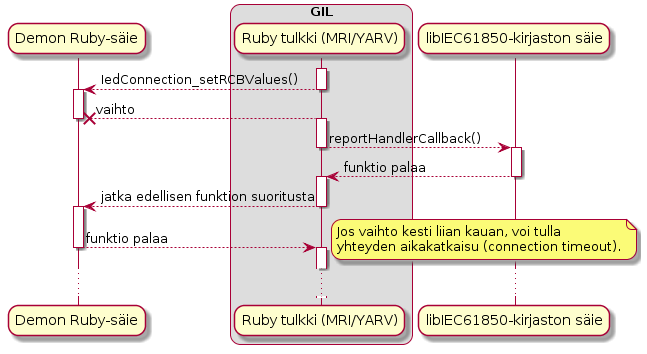
\includegraphics[width=1\textwidth]{pictures/ruby-gil.png}
	\caption{Ruby-tulkin globaalin lukituksen toiminta, joka vuorottaa ajossa olevia säikeitä riippumatta käyttöjärjestelmän vuorottajasta.}
	\label{fig:ruby-gil}
\end{figure}

Edellä mainittujen lisäksi demototeutuksessa oli muistivuoto huonon ohjelmoinnin takia. Muistivuoto on tilanne missä ohjelma varaa lisää muistia ilman, että sitä vapautetaan takaisin käyttöjärjestelmälle. Muistivuoto johtui todennäköisesti ohjelmointivirheestä ruby-ffi -kirjastolla. Kun liitos Rubysta tehdään C-kieleen, täytyy ohjelmoijan miettiä varatun muistin vapauttamista. Ruby-ohjelmoijan ei normaalisti tarvitse tästä huolehtia automaattisen roskien keruun ansiosta. Muistivuoto havaittiin kun ohjelma jätettiin suoritukseen pitemmäksi aikaa ja se oli varannut melkein kaiken käyttöjärjestelmän muistista itselleen. Tämän pystyi havaitsemaan helposti ohjelman suorituksen aikana Linuxin htop-ohjelmalla MEM\%-sarakkeesta. Sarake kertoo prosessin käyttämän prosentuaalisen osuuden koko käyttöjärjestelmän muistista \cite{htop-user-guide}. Luku kasvoi tasaisesti ja sen verran nopeasti, että sen havaitseminen oli mahdollista ilman pitempää suoritusaikaa.


\section{Yhteenveto}
Demon jatkokehitys toimivaksi olisi vaatinut paljon vaivaa huomioon ottaen tässä kappaleessa käsitellyt ongelmat. Tämän lisäksi sen kehityksessä ei oltu huomioitu järjestelmään hajautuksen vaatimuksia. Tiedon jakaminen muun järjestelmän kanssa tietokannan kautta ei ole hyvä ratkaisu. Se johtaisi tilanteeseen missä järjestelmän komponentit lukisivat viestejä tietokannasta jatkuvasti, ilman tietoa milloin uusi viesti on saapunut. Tästä aiheutuu turhaa kuormaa tietokannalle ja komponentin saama tieto ei välttämättä ole ajan tasalla. Isoilla muutoksilla demo olisi ollut mahdollista saada täyttämään asetetut vaatimukset ja sen ongelmat korjattua. Demo kuitenkin päätettiin korvata kokonaan uudella toteutuksella sen vaatiman työmäärän takia.

Ohjelmiston huonoon suorityskykyyn ja epävarmuuteen pääasiassa on syynä Ruby-kielen GIL ja suorituskyky tulkattavana kielenä. Varatun muistin määrän oli suuri yksinkertaista ohjelman ajamista varten. Syynä todennäköisesti oli RoR-kehyksen ajoympäristö, joka latasi muistiin muuta järjestelmää ja sen kirjastoja. Ohjelmassa oli muistivuoto, joka todennäköisesti johtui Ruby:n ja C-kielen liitoksen huonosta ohjelmoinnista. Edelle mainittuja tietoja käytetään apuna suunnittelussa esimerkiksi tekniikoiden valinnassa. Demototeutuksen perusteella libIEC61850-kirjasto todettiin hyväksi ja sitä tultiin käyttämään myös uudessa versiossa. Suunnitelussa kysymyksenä jää miettiä mitkä tekniikat valitaan toteutukseen, jotta suorituskykyongelmat vältetään ja varattu muisti pidetään pienenä. Muistivuoto ohjelmassa taas vältetään huolellisella ohjelmoinnilla.